\documentclass[12pt, a4paper]{article}
\usepackage[utf8]{inputenc}
\usepackage[top=2.5cm, bottom=2.5cm, left=3cm, right=3cm]{geometry}
\usepackage{tgschola}
\usepackage{listings}
\usepackage{graphicx}
\usepackage{hyperref}

\lstset{%
    basicstyle=\small\ttfamily,
    columns=flexible,
    frame=single,
    breaklines=true
}

\title{The Banzai Pipeline}
\author{Jibril Saffi}

\begin{document}
\maketitle

This project is a small mockup of a tool to build training pipelines for machine learning.
In the following report I'll try and explain some its features and the motivation behind them.

This is, of course, a quite limited example and though I tried to make sense of it as if it were
real, some of the design choices, such as implementing everything in a scripting language or the
lack of strictly defined API contracts, are compromised to the idea of a prototype.

\section{Three tiers}

\begin{figure}[htpb]
    \centering
    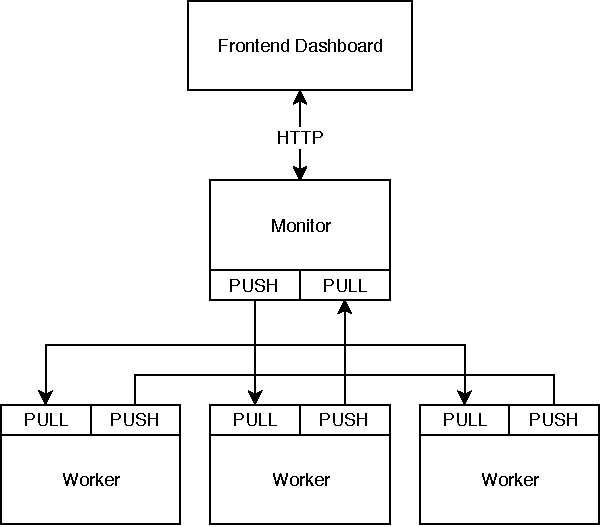
\includegraphics[width=0.6\linewidth]{arch.pdf}
    \caption{The gist of the architecture}
\end{figure}

The proposed architecture somewhat resembles the canonical three tier pattern.
Although it doesn't have a database layer per se, it does separates concerns into three.

The presentation, here of the progress and status of pipeline tasks, is handled by the dashboard, a React web page.

The decision making is handled by a tiny REST API allowing the user to create dashboards or inspect
their state through direct requests as well as through the aforementioned web page using a unified interface.

The actual pipeline tasks are executed by workers, multiple of which can run simultaneously on different machines.

\section{Pipelines are just lists of tasks}

Configuring a modular pipeline of tasks is both very generic and generally useful, and as such
there is a lot of previous work addressing the topic.
Multiple languages and tools have been specified to great lengths to do such a thing,
and though it would be interesting to delve into it, I chose not to.

In this example, a pipeline is only an ordered list of tasks.
And each task is an RPC call, with the input of the previous task as an implicit argument.
\begin{figure}[htpb]
    \centering
    \begin{lstlisting}
[
    {
        "call":"FETCH_FESTVOX",
        "args":[
          "http://festvox.org/cmu_arctic/cmu_arctic/packed/cmu_us_awb_arctic-0.90-release.zip"
        ]
    },{
        "call":"FILTER_LONGER",
        "args":[5]
    },{
        "call":"EXTRACT_MFCC",
        "args":[32,24,1,8000,16000]
    },{
        "call":"LEARN",
        "args":[]
    }
]
    \end{lstlisting}
    \caption{A pipeline, represented in JSON}
\end{figure}

This approach does have some limitations, for instance we can't represent multiples streams of data
in a single pipeline. And tasks within a pipeline can't be executed in parallel.
This is sufficient for our purposes, but we might benefit from a more complex model, such as a directed graph.

I chose not to bind the architecture too much by that model,
and since tasks are independently executable and modeled as simple RPCs, swapping in another pipeline model is not too difficult.

\section{Delegating messages to the network layer}

The scheduling and communication between the monitor and the workers is, in this example, delegated
to the network in the form of ZeroMQ PUSH and PULL sockets following the Pipeline pattern.
This communication takes the form of JSON messages as task orders and task reports.


In effect, this allows us to easily swap out our task scheduling mechanism by changing the routing
of those messages, without having to alter the logic of our code.

This has the quite desirable advantage of decoupling pipelines from tasks.
One can certainly imagine a scenario with specialized hardware for certain tasks. And scheduling tasks to run on
the machines where they will be most efficiently run is achievable with trivial alterations to the proposed architecture.

\section{Decoupling data from process}

Given we are working on audio datasets with heavy files, passing the entire dataset and results around is not advisable, for many reasons.
Decoupling the semantic representation of data from the actual contents of the dataset is therefore profitable.

This is easily solved by passing identifiers for the data of course, but simply using arbitrary identifiers has pitfalls.
We would like to retain the ability to cache tasks, our tasks being mostly deterministic.
Content
addressing\footnote{\url{https://en.wikipedia.org/wiki/Content-addressable_storage}} is very useful in this instance, using a hash of said WAV file we can ensure that
we are talking about the same file with acceptable probability, and handle it accordingly.

\section{Distributed data distribution}

Still, there is the problem of actually getting data from one task to the other, which is non-trivial if we pose the constraint
of having tasks run on arbitrary machines. Content addressing is also useful here. Using IPFS, we can
treat that file hash as a universal handle, usable on any machine and the associated data will be
transfered and resolved seamlessly through the network, with a small overhead.

Indeed, a more centralized approach would have been to use a centralized datastore for this
purpose, which has some advantages (archival or authoritative changes are easier for instance)
but fetching from a single point can also be a problem.

We don't want to assume that every worker will be close (geographically or in terms of network) to
such a store and it seems like a better idea to just fetch from the closest person to have our data.
In the best case, they might be one of our neighbour workers, who just recently processed that same data.

In this context, a distributed solution, such as the one provided by IPFS in the form of a DHT is far better.
We just resolve who is the closest person to have the data behind a certain hash, and fetch from them.

This has the positive side effect of providing our users with a unified way to access and share
their dataset and all the intermediary and final results of their computations.
All of which can be seamlessly implemented inside the browser.

\end{document}
